Устройство управления представляет собой интерфейс узла, через который осуществляется всё взаимодействие с внешним миром. УУ состоит из селектора адреса (CА) и конечного автомата управления (КАУ). Селектор адреса (СА) читает шину адреса (ША) и при поступлении адреса из нужного диапазона (0x30-0x35) формирует сигнал разрешения. При разрешении от СА, КАУ может работать. КАУ читает шину управления (ШУ) - 2 разряда - и реагирует на следующие сигналы от неё:
\begin{description}
\item[01] Сигнал START. УУ запускается, считывает режим работы из адреса в регистр режима и подаёт разрешающий сигнал на формирователь импульсной последовательности.
\item[10] Сигнал READ. Реакция на этот сигнал будет только при условии, что ранее подавался сигнал START, т.е. УУ запущено. При поступлении данного сигнала, УУ считывает три разряда из регистра режима и подаёт их на шину данных.
\item[11] Сигнал STOP. Реакция на этот сигнал будет только при условии, что ранее подавался сигнал START, т.е. УУ запущено. При поступлении данного сигнала, УУ перестаёт подавать разрешающий сигнал на формирователь импульсной последовательности и подаёт сигнал синхронного сброса на регистр режима. После этого УУ считается выключенным.
\end{description}

Режим работы формирователя импульсной последовательности передаётся в младших трёх битах 8-битного адреса, по ША, как часть адреса. В таблице \ref{table:modes} приведено соответствие между адресами и выходными импульсными последовательностями.

\begin{table}[h]
  \centering
  \begin{tabular}{|l|l|l|}
    \hline
    Адрес & Номер режима & Выходная последовательность импульсов \\ \hline
    0x30 & 1 & 3, 8, 11, 20 \\ \hline
    0x31 & 2 & 2, 4, 12, 21 \\ \hline
    0x32 & 3 & 5, 10, 15, 16 \\ \hline
    0x33 & 4 & 8, 9, 13, 17 \\ \hline
    0x34 & 5 & 1, 6, 11, 19 \\ \hline
    0x35 & 6 & 1, 2, 7, 9, 18, 22 \\ \hline
  \end{tabular}
  \caption{Соответствие адресов различным режимам}
  \label{table:modes}
\end{table}

Селектор адреса представляет собой простой элемент И, входами которого являются разряды адреса. Функциональная схема селектора адреса приведена на рис. \ref{fig:selector}.

\begin{figure}
  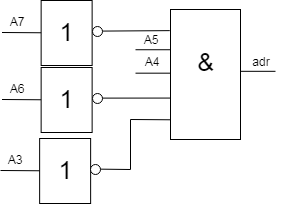
\includegraphics[scale=1]{./selector.png}
  \caption{Функциональная схема селектора адреса}
  \label{fig:selector}
\end{figure}

Конечный автомат управления представляет из себя конечный автомат Мура, генерирующий управляющие сигналы и коммутирующий потоки данных. Автомат описан таблицей \ref{table:auto}. Функциональная схема конечного автомата управления приведена на рис. \ref{fig:fca}.

\begin{table}[h]
  \centering
  \begin{tabular}{|c|c|c|c|c|c|c|}
    \hline
    \multicolumn{3}{|c|}{Состояние}  &  Условие перехода & \multicolumn{3}{|c|}{Переход в} \\ \cline{1-3} \cline{5-7}
    Q3 & Q1 & Q0 & & Q3 & Q1 & Q0 \\ \hline
    0  & 0 & 0 & adr \& start & 0 & 0 & 1\\ \cline{4-7}
                                     &  &  &  \textoverline{adr \& start} & 0 & 0 & 0 \\ \hline
    0 & 0 & 1 & 1 & 0 & 1 & 0 \\ \hline
    0 & 1 & 0 & adr \& stop  & 1 & 0 & 0 \\ \cline{4-7}
                                     &  &  & adr \& rd & 0 & 1 & 1 \\ \cline{4-7}
                                     &  &  &  \textoverline{adr \& stop}  & 0 & 1 & 0 \\ \cline{4-7}
                                     &  &  &  \textoverline{adr \& rd} & 0 & 1 & 0 \\ \hline
    1 & 0 & 0 & 1 & 0 & 0 & 0 \\ \hline
    0 & 1 & 1 & 1 & 0 & 1 & 0 \\ \hline
  \end{tabular}
  \caption{Структурная таблица конечного автомата}
  \label{table:auto}
\end{table}

\begin{figure}
  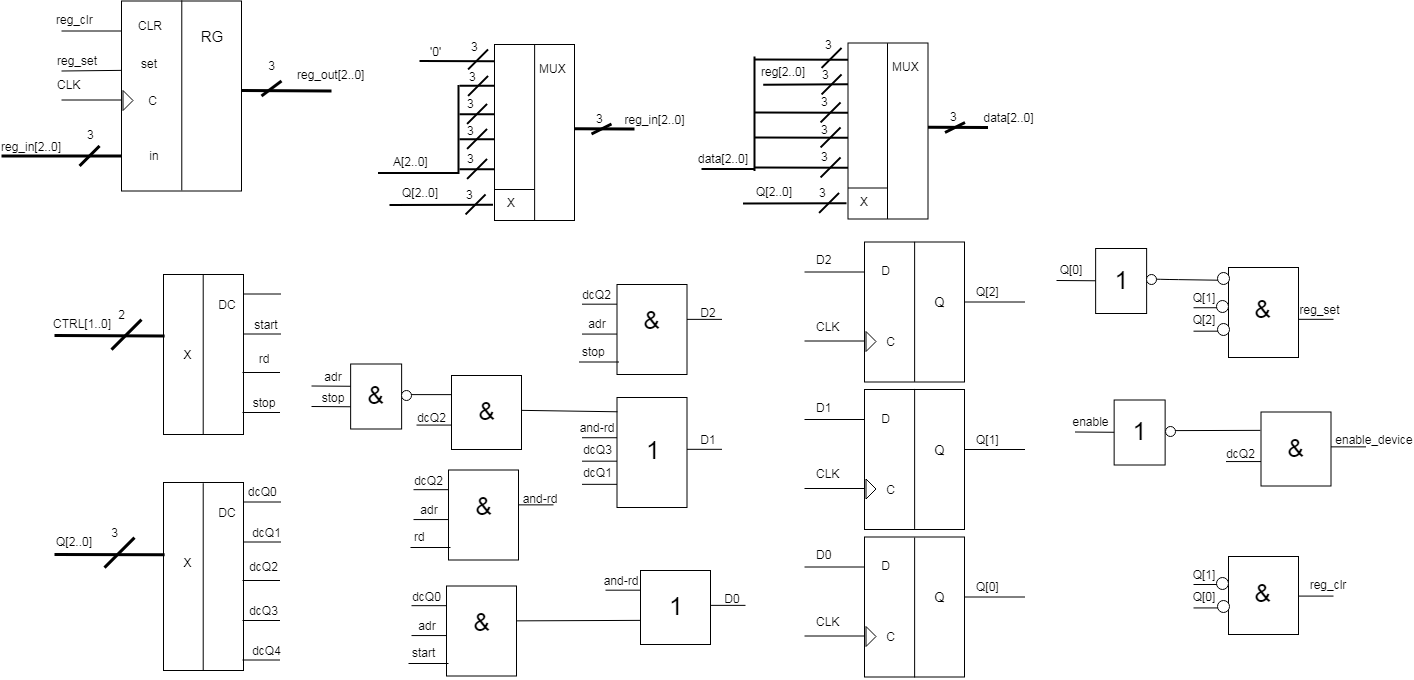
\includegraphics[scale=0.35]{./FCA.png}
  \caption{Функциональная схема }
  \label{fig:fca}
\end{figure}